\newpage
\section{energyLIVE API Specification}
\label{appendix:energylive-api}

The energyLIVE API, provided by Energie Steiermark, enables the integration of real-time smart meter data into third-party systems, thereby supporting advanced energy management and automation solutions. This interface is designed to facilitate the retrieval of consumption data and system status from smart meters, and can be combined with the smartENERGY electricity price API for dynamic tariff applications such as smartCONTROL.

\subsection{Authentication and Access}

Access to the energyLIVE API requires authentication via an HTTPS header, specifically the \texttt{X-API-KEY}, which must contain a valid key obtained from the customer portal. All requests must be made over secure HTTPS connections to ensure data privacy and integrity.

\subsection{Base URL and Endpoints}
The base URL for the API is:
\begin{quote}
    \url{https://backend.energylive.e-steiermark.com/api/v1/}
\end{quote}
To retrieve the latest measurements from a specific smart meter interface, the following endpoint is used:
\begin{quote}
    \texttt{devices/I-XXXXXXXX-XXXXXXXX/measurements/latest}
\end{quote}
where the interface UID is provided by the customer portal.

\subsection{Data Format and Response Structure}
API responses are returned in JSON format, consisting of an array of measurement objects. Each object contains the following fields:
\begin{itemize}
    \item \textbf{measurement}: Specifies the type of value, typically indicated by an OBIS code for electrical quantities.
    \item \textbf{timestamp}: The time at which the measurement was recorded in the energyLIVE database, represented as a 13-digit Unix timestamp (milliseconds).
    \item \textbf{value}: The measured value, with units such as watt-hours (Wh) for meter readings and watts (W) for instantaneous power.
\end{itemize}

\subsection{Example Request and Response}
A typical request to the API using \texttt{curl} is as follows:
\begin{lstlisting}
curl -X GET -H "X-API-KEY: <your_api_key>" \
"https://backend.energylive.e-steiermark.com/api/v1/devices/I-10082023-01658401/measurements/latest"
\end{lstlisting}

The response is a JSON array, for example:
\begin{lstlisting}
[
  {
    "measurement": "0100010700",
    "timestamp": 1726559995000,
    "value": 138.0
  },
  {
    "measurement": "0100010800",
    "timestamp": 1726559995000,
    "value": 9577201.0
  }
  // ...
]
\end{lstlisting}

\subsection{Use Cases}
The energyLIVE API is suitable for a variety of applications, including the integration of smart meter data into home automation platforms, the development of custom energy monitoring dashboards, and the implementation of dynamic energy management strategies based on real-time consumption and pricing data.

For further details and best practice examples, refer to the official documentation and user community resources provided by Energie Steiermark\footnote{\url{https://www.smartenergy.at/api-schnittstelle-energylive}}.

\newpage
\section{smartENERGY Strompreis API Specification}
\label{appendix:strompreis-api}

The smartENERGY Strompreis API, provided by Energie Steiermark, enables customers to access quarter-hourly electricity price data in real time, facilitating the integration of dynamic pricing information into custom systems and applications. This API supports the automation of energy consumption and the optimization of energy management strategies by providing timely and accurate market price data from the EPEX Spot AT electricity exchange.

\subsection{Authentication and Access}
The Strompreis API is publicly accessible and does not require authentication or special parameters for basic price retrieval. All requests are made via HTTPS to ensure secure data transmission.

\subsection{Base URL and Endpoint}
The base URL for the API is:
\begin{quote}
    \url{https://apis.smartenergy.at/market/v1/price}
\end{quote}
A simple GET request to this endpoint returns the latest available electricity price data.

\subsection{Data Format and Response Structure}
The API returns data in JSON format, with the following structure:
\begin{itemize}
    \item \textbf{tariff}: The tariff identifier, typically set to \texttt{EPEXSPOTAT}.
    \item \textbf{unit}: The unit of the price value, e.g., \texttt{ct/kWh}.
    \item \textbf{interval}: The validity interval of each price entry in minutes (usually 15).
    \item \textbf{data}: An array of objects, each containing:
    \begin{itemize}
        \item \textbf{date}: The local date and time from which the price is valid.
        \item \textbf{value}: The price including 20\% VAT, in decimal format.
    \end{itemize}
\end{itemize}

\subsection{Example Request and Response}
A typical request to the API is as follows:
\begin{lstlisting}
GET https://apis.smartenergy.at/market/v1/price
\end{lstlisting}

The response is a JSON object, for example:
\begin{lstlisting}
{
  "tariff": "EPEXSPOTAT",
  "unit": "ct/kWh",
  "interval": 15,
  "data": [
    {
      "date": "2023-06-23T00:00:00+02:00",
      "value": 12.592
    },
    ...
  ]
}
\end{lstlisting}

\subsection{Use Cases}
The Strompreis API is particularly useful for automating energy consumption in response to real-time price signals, enabling the development of energy management systems that optimize usage patterns according to periods of low electricity prices. It also supports detailed energy monitoring and cost analysis by providing granular, up-to-date market price data.

For further details and best practice examples, refer to the official documentation and user community resources provided by Energie Steiermark\footnote{\url{https://www.smartenergy.at/api-schnittstellen}}.

\newpage
\section{Tasmota Configuration for NOUS A5T Power Strip}
\label{appendix:tasmota-config}

This appendix details the custom Tasmota configuration used for the NOUS A5T power strip, enabling secure integration with AWS IoT and advanced energy monitoring capabilities. The configuration is designed to facilitate reproducibility and ease of deployment for research and practical applications in energy-aware server management.

\subsection{Hardware Overview}
The NOUS A5T power strip features four individually controllable AC outlets, three USB ports, and integrated energy monitoring for voltage, current, and power. The device is based on the ESP8285 microcontroller, which provides 1MB of flash memory and supports custom firmware such as Tasmota.

\subsection{Configuration Purpose and Features}
The custom configuration enables the following key features:
\begin{itemize}
    \item Secure AWS IoT integration with TLS/SSL support
    \item MQTT communication for real-time telemetry
    \item Energy monitoring (voltage, current, power)
    \item Custom device naming and topic structure
    \item Web interface and HTTP API for local management
    \item Rules engine for automation
\end{itemize}

\subsection{Device Template}
The following Tasmota template is used to define the hardware configuration for the NOUS A5T:
\begin{lstlisting}
{
  "NAME": "NOUS A5T",
  "GPIO": [0, 3072, 544, 3104, 0, 259, 0, 0, 225, 226, 224, 0, 35, 4704],
  "FLAG": 1,
  "BASE": 18
}
\end{lstlisting}

\subsection{Custom Firmware Build and Flashing}
To deploy the custom configuration, the following steps should be followed:
\begin{enumerate}
    \item Copy the provided \texttt{user\_config\_override.h} file to the Tasmota source directory:
    \begin{lstlisting}
    copy tasmota-config\user_config_override.h tasmota\tasmota\user_config_override.h
    \end{lstlisting}
    \item Build the custom firmware using PlatformIO:
    \begin{lstlisting}
    cd tasmota
    pio run -e tasmota
    \end{lstlisting}
    \item Flash the firmware to the NOUS A5T device. The built binary is located at \lstinline|tasmota/build_output/firmware/tasmota.bin|. Flashing can be performed via the Tasmota web UI or a serial connection.
\end{enumerate}

\subsection{AWS IoT and MQTT Setup}
After flashing, configure the device for AWS IoT integration using the following Tasmota console command (replace placeholders with your actual AWS IoT endpoint and credentials):
\begin{lstlisting}
BackLog SetOption3 1; SetOption103 1; MqttHost your-endpoint.iot.region.amazonaws.com; MqttPort 443; MqttUser tasmota?x-amz-customauthorizer-name=TasmotaAuth; MqttPassword your-password
\end{lstlisting}

\subsection{Device Information}
\begin{itemize}
    \item \textbf{Name}: Server PowerMeter
    \item \textbf{Topic}: serverpowermeter
    \item \textbf{Firmware}: Custom Tasmota v14.6.0 with AWS IoT support
\end{itemize}

For further details, refer to the configuration file \texttt{user\_config\_override.h} and the project README. This setup enables secure, scalable, and reproducible energy monitoring for research and operational deployments.

\newpage
\section{DynamoDB Cleanup Script: deleteTimestamps.py}
\label{appendix:delete-timestamps}

This appendix documents the Python script \texttt{deleteTimestamps.py}, which is used to clean up the DynamoDB \texttt{SensorData} table by deleting items with timestamps that do not include microseconds. This operation is necessary after migrating to a new timestamp format to ensure data consistency and prevent legacy entries from affecting subsequent analyses.

\subsection{Purpose and Functionality}
The script scans the \texttt{SensorData} table for items whose timestamp attribute (used as the sort key) is exactly 19 characters long, indicating the absence of microseconds. It then interactively deletes these items, using both the partition key and sort key for precise targeting. The script employs exponential backoff to handle DynamoDB throughput limits and provides progress updates during both scanning and deletion phases.

\subsection{Prerequisites}
\begin{itemize}
    \item Python 3.x
    \item \texttt{boto3} and \texttt{botocore} libraries installed (\texttt{pip install boto3 botocore})
    \item AWS credentials configured with permissions to read and delete from the \texttt{SensorData} table
\end{itemize}

\subsection{Usage Instructions}
\begin{enumerate}
    \item Ensure your AWS credentials are set up (e.g., via \texttt{aws configure} or environment variables).
    \item Run the script in a terminal:
    \begin{lstlisting}
    python deleteTimestamps.py
    \end{lstlisting}
    \item Review the summary of items to be deleted and confirm when prompted.
    \item The script will delete the identified items, providing progress updates.
\end{enumerate}

\subsection{Script Listing}
The full source code is provided below for reproducibility:
\begin{lstlisting}[language=Python]
# This script is used to delete items from the SensorData table that have a timestamp 
# without microseconds.
# It is used to clean up the table after the migration to the new format.

import boto3
import time
from botocore.exceptions import ClientError

# Initialize DynamoDB
dynamodb = boto3.resource('dynamodb')
table = dynamodb.Table('SensorData')

print("Checking table schema...")

# Get table description to find primary key
table_description = table.meta.client.describe_table(TableName='SensorData')
key_schema = table_description['Table']['KeySchema']

print("Table key schema:")
for key in key_schema:
    print(f"  {key['AttributeName']} ({key['KeyType']})")

# Find the partition key and sort key
partition_key_name = None
sort_key_name = None
for key in key_schema:
    if key['KeyType'] == 'HASH':  # Partition key
        partition_key_name = key['AttributeName']
    elif key['KeyType'] == 'RANGE':  # Sort key
        sort_key_name = key['AttributeName']

if not partition_key_name or not sort_key_name:
    print("ERROR: Could not find partition key or sort key")
    exit(1)

print(f"Partition key: {partition_key_name}")
print(f"Sort key: {sort_key_name}")

print("Scanning DynamoDB table...")

# Count items without microseconds
count_without_microseconds = 0
items_to_delete = []
total_scanned = 0

def scan_with_retry(exclusive_start_key=None):
    """Scan with exponential backoff for throughput exceptions"""
    max_retries = 5
    base_delay = 1
    
    for attempt in range(max_retries):
        try:
            if exclusive_start_key:
                response = table.scan(
                    ExclusiveStartKey=exclusive_start_key,
                    ProjectionExpression='#pk, #sk',
                    ExpressionAttributeNames={
                        '#pk': partition_key_name, 
                        '#sk': sort_key_name
                    }
                )
            else:
                response = table.scan(
                    ProjectionExpression='#pk, #sk',
                    ExpressionAttributeNames={
                        '#pk': partition_key_name, 
                        '#sk': sort_key_name
                    }
                )
            return response
        except ClientError as e:
            if e.response['Error']['Code'] == 'ProvisionedThroughputExceededException':
                if attempt < max_retries - 1:
                    delay = base_delay * (2 ** attempt)  # Exponential backoff
                    print(f"Throughput exceeded, waiting {delay} seconds...")
                    time.sleep(delay)
                else:
                    raise
            else:
                raise

# Scan with pagination to get all items
try:
    response = scan_with_retry()
    
    # Process first batch
    for item in response['Items']:
        total_scanned += 1
        timestamp = item[sort_key_name]  # Use sort key name
        if len(timestamp) == 19:  # No microseconds
            count_without_microseconds += 1
            # Use both partition key and sort key for deletion
            delete_key = {
                partition_key_name: item[partition_key_name],
                sort_key_name: item[sort_key_name]
            }
            items_to_delete.append(delete_key)
    
    # Continue scanning while there are more items
    while 'LastEvaluatedKey' in response:
        print(f"Scanned {total_scanned} items so far...")
        time.sleep(0.1)  # Small delay between scans
        
        response = scan_with_retry(response['LastEvaluatedKey'])
        
        for item in response['Items']:
            total_scanned += 1
            timestamp = item[sort_key_name]  # Use sort key name
            if len(timestamp) == 19:  # No microseconds
                count_without_microseconds += 1
                # Use both partition key and sort key for deletion
                delete_key = {
                    partition_key_name: item[partition_key_name],
                    sort_key_name: item[sort_key_name]
                }
                items_to_delete.append(delete_key)

except ClientError as e:
    if e.response['Error']['Code'] == 'ProvisionedThroughputExceededException':
        print("ERROR: DynamoDB throughput exceeded. Consider:")
        print("1. Increasing provisioned throughput")
        print("2. Running this script during off-peak hours")
        print("3. Using on-demand billing mode")
    else:
        print(f"ERROR: {e.response['Error']['Message']}")
    exit(1)

print(f"Total items scanned: {total_scanned}")
print(f"Found {count_without_microseconds} items without microseconds")

if count_without_microseconds > 0:
    # Show first few items to delete
    print("First 5 items to delete:")
    for item in items_to_delete[:5]:
        print(f"  {item}")
    
    # Ask for confirmation
    confirm = input("Do you want to delete these items? (yes/no): ")
    if confirm.lower() == 'yes':
        # Delete items with rate limiting
        deleted_count = 0
        for item in items_to_delete:
            try:
                table.delete_item(Key=item)
                deleted_count += 1
                if deleted_count % 50 == 0:  # Progress update every 50 items
                    print(f"Deleted {deleted_count} items...")
                    time.sleep(0.1)  # Small delay
            except ClientError as e:
                if e.response['Error']['Code'] == 'ProvisionedThroughputExceededException':
                    print(f"Throughput exceeded while deleting. Stopped at {deleted_count} items.")
                    break
                else:
                    print(f"Error deleting item: {e.response['Error']['Message']}")
        print(f"Successfully deleted {deleted_count} items")
    else:
        print("Deletion cancelled")
else:
    print("No items found without microseconds")
\end{lstlisting}

\newpage
\section{AWS QuickSight Dashboard Configuration}
\label{appendix:quicksight-dashboard}

This appendix documents the configuration of the AWS QuickSight dashboards used for energy consumption and price analysis. The dashboards visualize data from smart meters, server sensors, and the EPEX Spot electricity market, enabling comprehensive monitoring and analysis.

\subsection{QuickSight Data Preparation}
The following custom SQL queries were used in Amazon Athena to prepare the data for visualization:

\paragraph{Energy Consumption (energyLIVE)}
\begin{lstlisting}[language=SQL]
SELECT
    value AS W_Complete,
    timestamp,
    unit,
    from_unixtime(round(timestamp/1000/900)*900) AS interval_15min
FROM "Athena-esoxvek5"."default"."energylivedata"
WHERE unit = 'W'
  AND value IS NOT NULL
  AND value > 0
\end{lstlisting}

\paragraph{Sensor Data (sensordata)}
\begin{lstlisting}[language=SQL]
SELECT
    *,
    date_trunc('minute', date_parse(device_time, '%Y-%m-%dT%H:%i:%s')) as interval_15min
FROM "Athena-esoxvek5"."default"."sensordata"
\end{lstlisting}

\subsection{Dashboard Visualizations}
The following figures show the main QuickSight dashboards used in this project:

% Energy Consumption Dashboard
\begin{figure}[H]
    \centering
    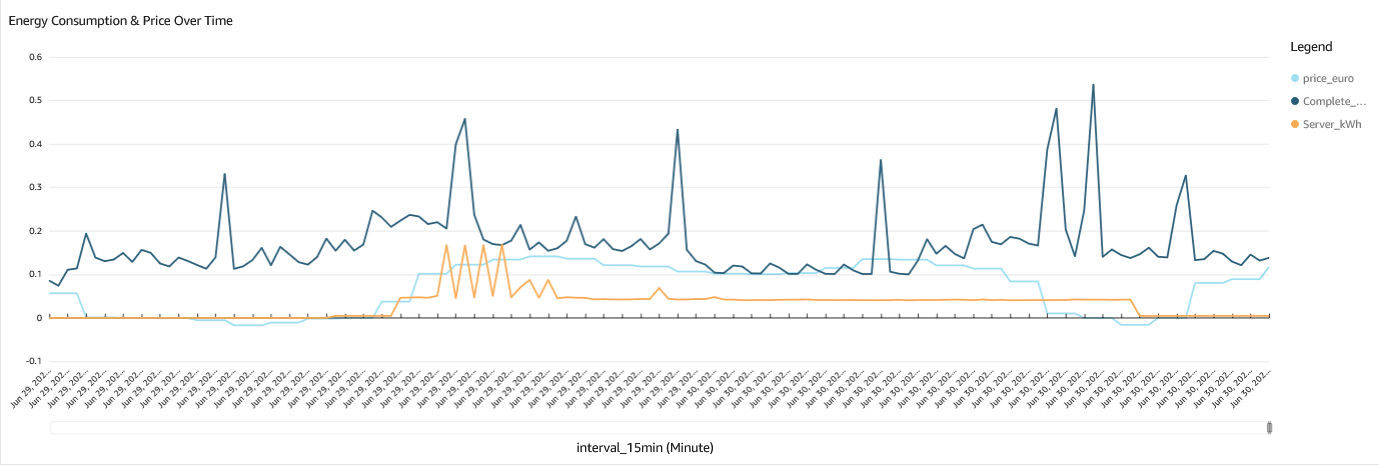
\includegraphics[width=0.95\textwidth]{fig/aggregated_Energyconsumption Dashboard.png}
    \caption{Aggregated Energy Consumption Dashboard}
\end{figure}

% Energy Live Data Preparation
\begin{figure}[H]
    \centering
    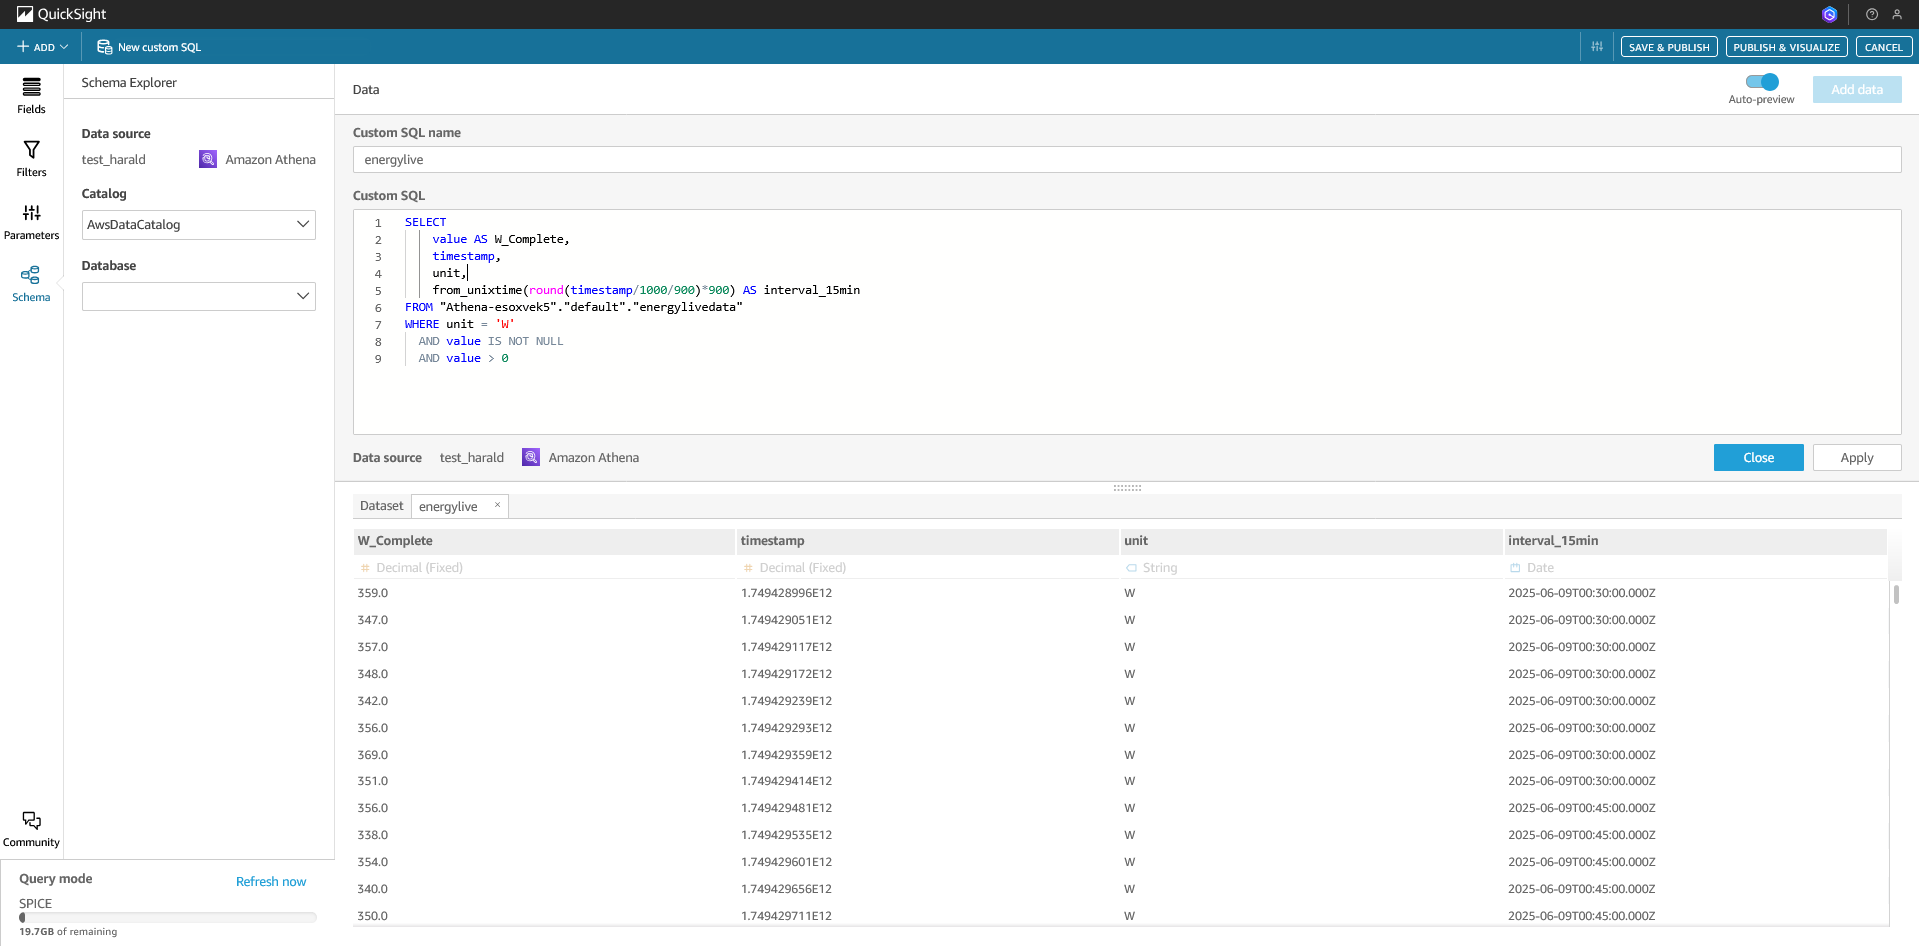
\includegraphics[width=0.95\textwidth]{fig/energylive_Data Prep.png}
    \caption{QuickSight Data Preparation for energyLIVE}
\end{figure}

% EPEX Price Dashboard
\begin{figure}[H]
    \centering
    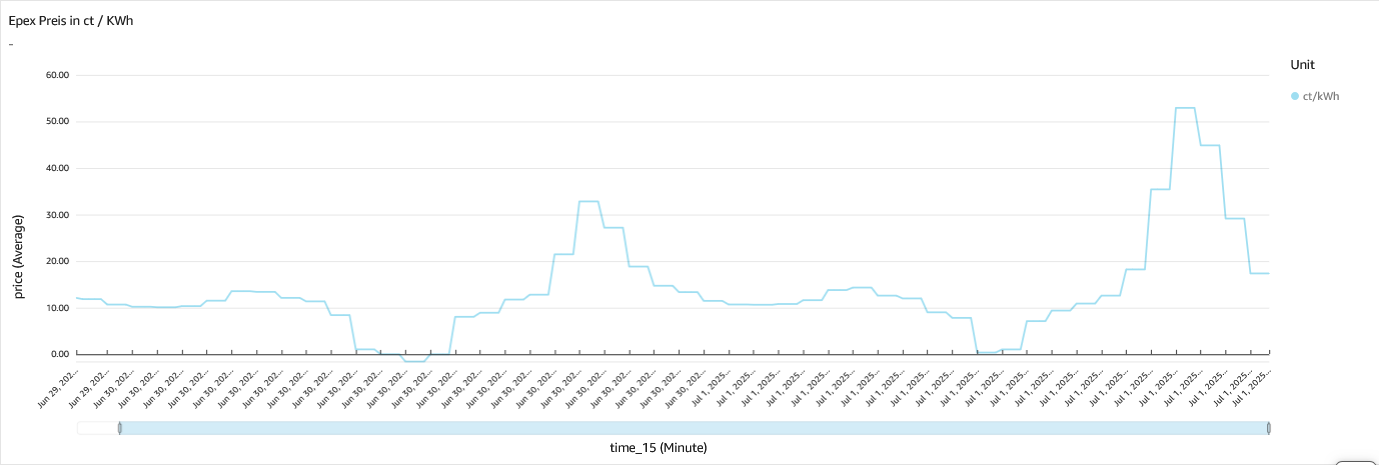
\includegraphics[width=0.95\textwidth]{fig/epex_Energyconsumption Dashboard.png}
    \caption{EPEX Price Dashboard}
\end{figure}

% Full Dashboard
\begin{figure}[H]
    \centering
    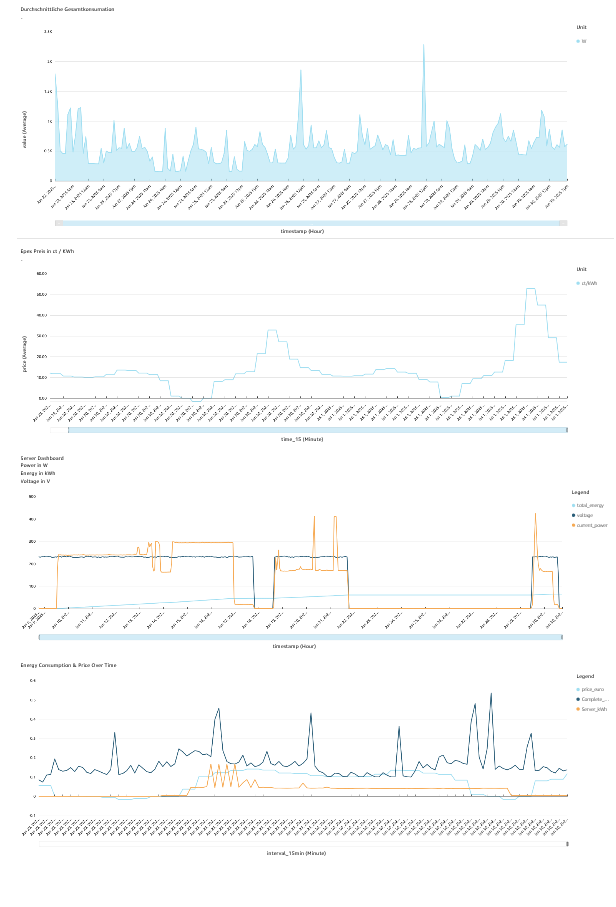
\includegraphics[width=0.95\textwidth]{fig/fulldashboardnergyconsumption Dashboard.png}
    \caption{Full Energy Consumption Dashboard}
\end{figure}

% Sensor Data Preparation
\begin{figure}[H]
    \centering
    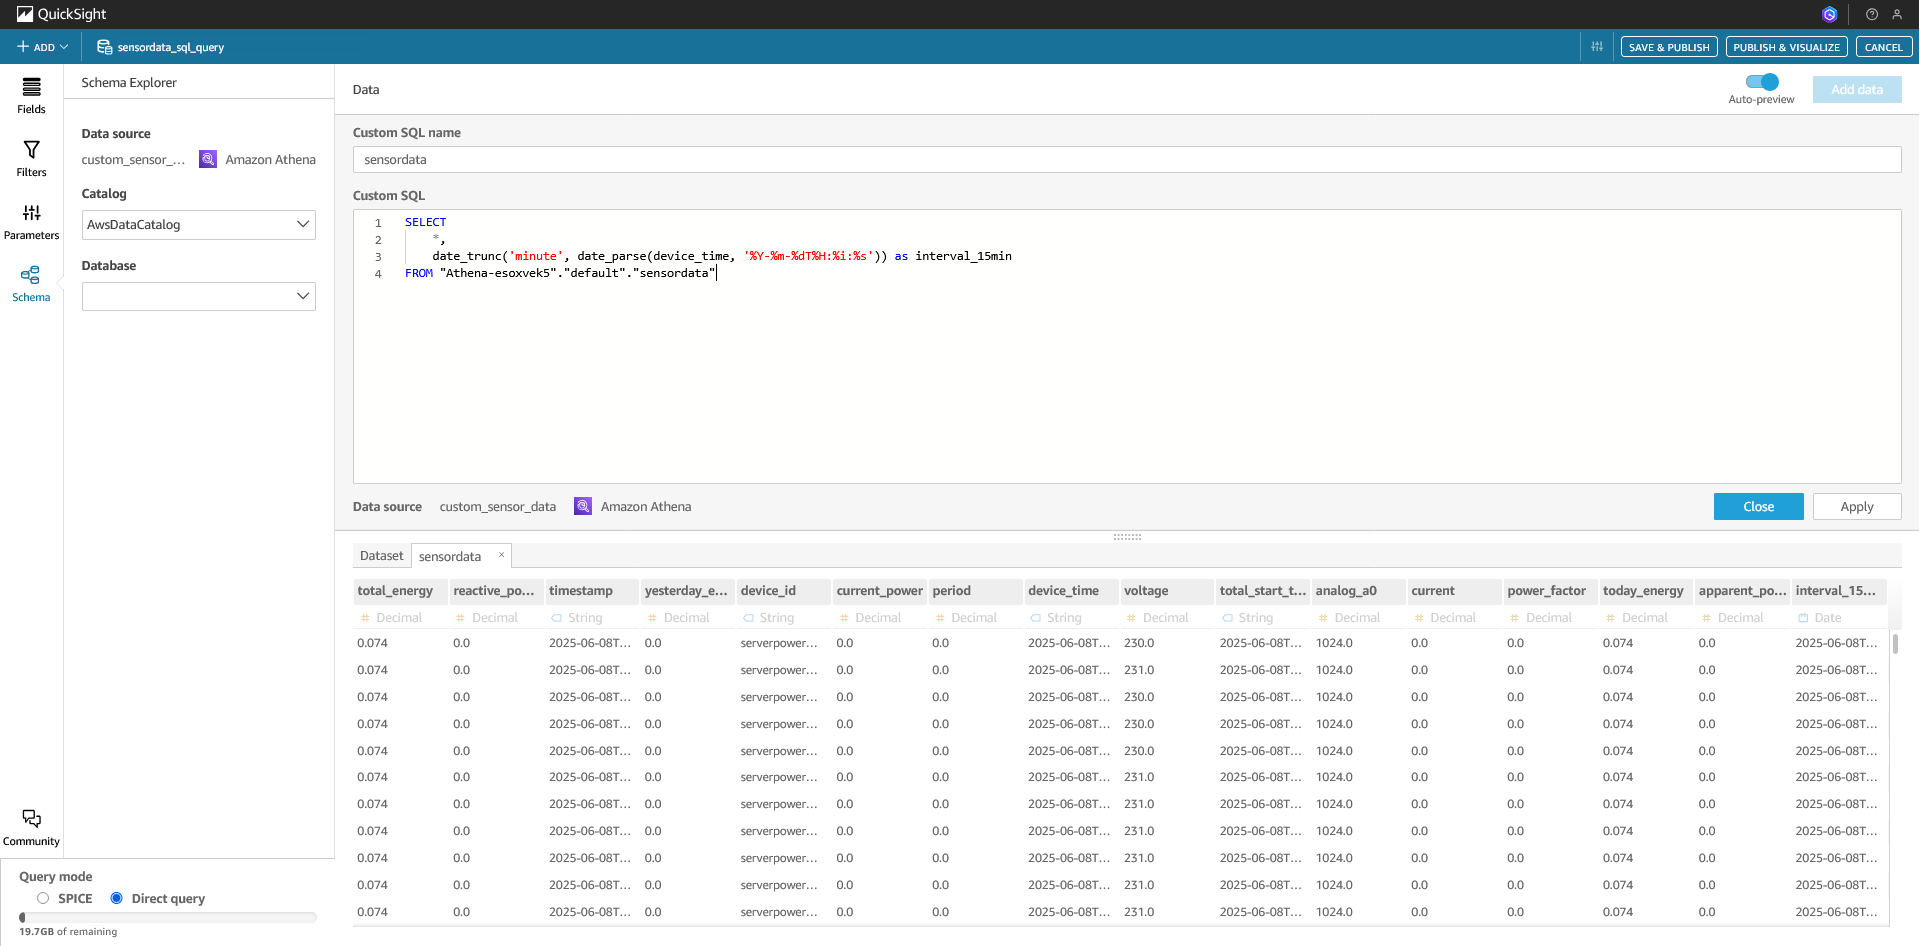
\includegraphics[width=0.95\textwidth]{fig/sensordata_Data Prep.png}
    \caption{QuickSight Data Preparation for Sensor Data}
\end{figure}

% Server Data Dashboard
\begin{figure}[H]
    \centering
    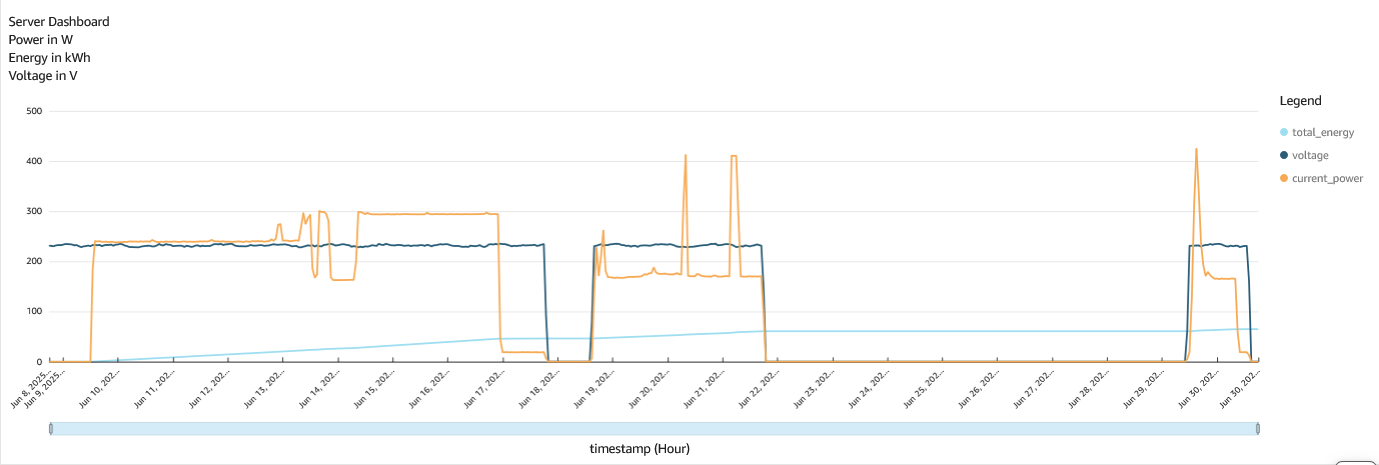
\includegraphics[width=0.95\textwidth]{fig/server_data_Energyconsumption Dashboard.png}
    \caption{Server Data Energy Consumption Dashboard}
\end{figure}

% Smart Meter Consumption Dashboard
\begin{figure}[H]
    \centering
    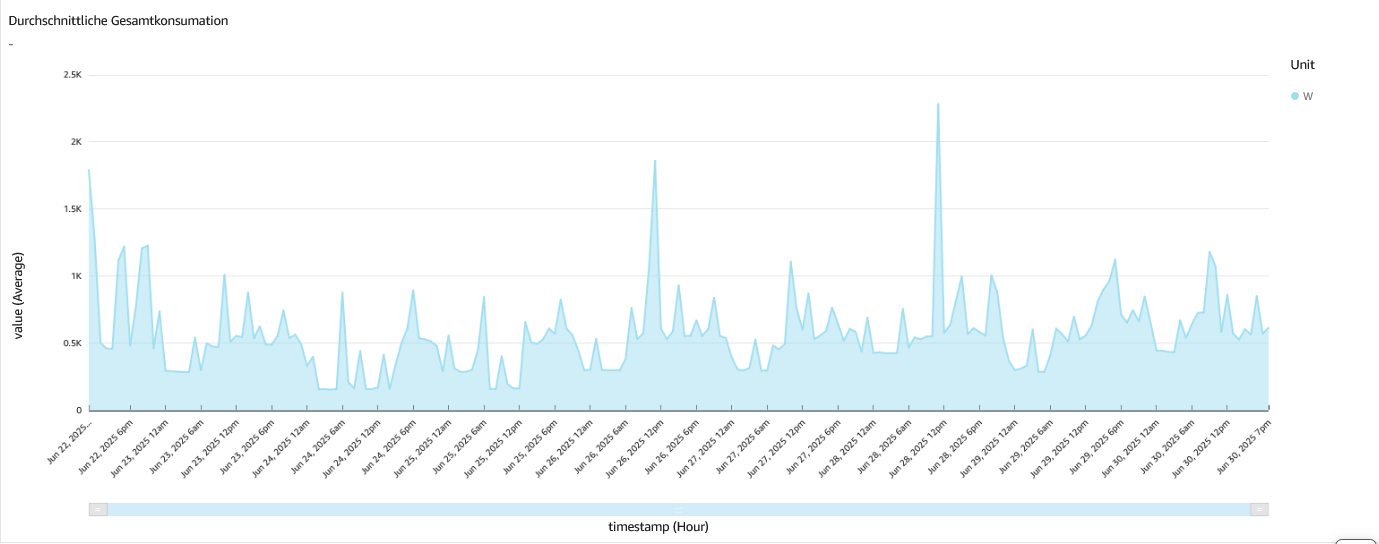
\includegraphics[width=0.95\textwidth]{fig/smart_meterconsumptionEnergyconsumption Dashboard.png}
    \caption{Smart Meter Consumption Dashboard}
\end{figure}

For further details on the QuickSight configuration and interactive dashboards, see the project presentation and the HTML presentation project documentation (Section~\ref{appendix:github-docs}).

\newpage
\section{GitHub Repository and Documentation}
\label{appendix:github-docs}

This appendix provides permanent references to the project's GitHub repository and its core documentation. The repository contains all source code, configuration files, and documentation required to replicate the research and implementation described in this paper.

\subsection{Repository Information}
\begin{itemize}
    \item \textbf{Repository URL}: \url{https://github.com/papers-mcce/energyops}
    \item \textbf{Main Branch}: \texttt{main}
    \item \textbf{Documentation Branch}: \texttt{final-paper}
\end{itemize}

\subsection{Core Documentation Structure}
The repository's documentation is organized hierarchically, with the main README.md serving as the entry point. Key documentation components include:

\subsubsection{Main Project Documentation}
The primary README.md (\url{https://github.com/papers-mcce/energyops/blob/main/README.md}) provides:
\begin{itemize}
    \item Project overview and objectives
    \item Complete directory structure
    \item Deployment instructions
    \item Configuration guides
    \item Replication procedures
\end{itemize}

\subsubsection{Component-Specific Documentation}
\begin{enumerate}
    \item \textbf{Terraform Infrastructure} \\
    \url{https://github.com/papers-mcce/energyops/blob/main/Deployment/terraform/README.md}
    \begin{itemize}
        \item AWS resource specifications
        \item Deployment procedures
        \item Security configurations
        \item Infrastructure diagrams
    \end{itemize}

    \item \textbf{Energy Analysis Tools} \\
    \label{appendix:energy-analysis}
    \url{https://github.com/papers-mcce/energyops/blob/main/Deployment/Energy-Analysis/README_energy_analysis.md}
    \begin{itemize}
        \item Data collection scripts
        \item Analysis methodologies
        \item Visualization tools
        \item Result interpretation guides
    \end{itemize}

    \item \textbf{Tasmota Configuration} \\
    \url{https://github.com/papers-mcce/energyops/blob/main/tasmota-config/README.md}
    \begin{itemize}
        \item Device setup instructions
        \item Custom firmware configuration
        \item AWS IoT integration steps
        \item Troubleshooting guides
    \end{itemize}

    \item \textbf{HTML Presentation} \\
    \url{https://github.com/papers-mcce/energyops/blob/main/html-presentation-project/README.md}
    \begin{itemize}
        \item Interactive visualization setup
        \item Deployment instructions
        \item Customization options
        \item Browser compatibility notes
    \end{itemize}
\end{enumerate}

\subsection{Cross-References and Dependencies}
The documentation maintains internal cross-references using LaTeX labels. Key references include:
\begin{itemize}
    \item Energy Analysis (Section~\ref{appendix:energylive-api})
    \item Price API Documentation (Section~\ref{appendix:strompreis-api})
    \item Device Configuration (Section~\ref{appendix:tasmota-config})
    \item Database Management (Section~\ref{appendix:delete-timestamps})
\end{itemize}

\subsection{Version Control and Updates}
The documentation is maintained under version control, with updates tracked through Git commits and pull requests. Major changes are documented in the repository's release notes and change logs.

For the most current version of any documentation component, refer to the repository URLs provided above. All links are permanent and reference specific commits to ensure reproducibility of the research implementation.

\section*{Reproducibility Note}
All scripts, infrastructure code, and setup guides referenced in this paper are included in the project materials to support full reproducibility of the research and experiments described.
